\subsection{Evaluación del Dashboard}

\subsection*{Descripción General}

El dashboard desarrollado con Streamlit, denominado \textit{Dashboard de URLs}, está diseñado para analizar y visualizar características de URLs almacenadas en la base de datos. El dashboard tiene dos partes principales:

\begin{enumerate}
    \item \textbf{Análisis de URL:} Permite a los usuarios ingresar una URL para obtener un informe detallado de sus características, incluyendo si es maligna o no. Este proceso toma aproximadamente 5 segundos.
    \item \textbf{Dashboard de Estadísticas:} Muestra diversas gráficas e informes sobre las características de las URLs almacenadas en la base de datos, ofreciendo una visión detallada y rápida de los datos ya extraídos.
\end{enumerate}

\subsection*{Funcionamiento}


\begin{figure}[H]
    \centering
    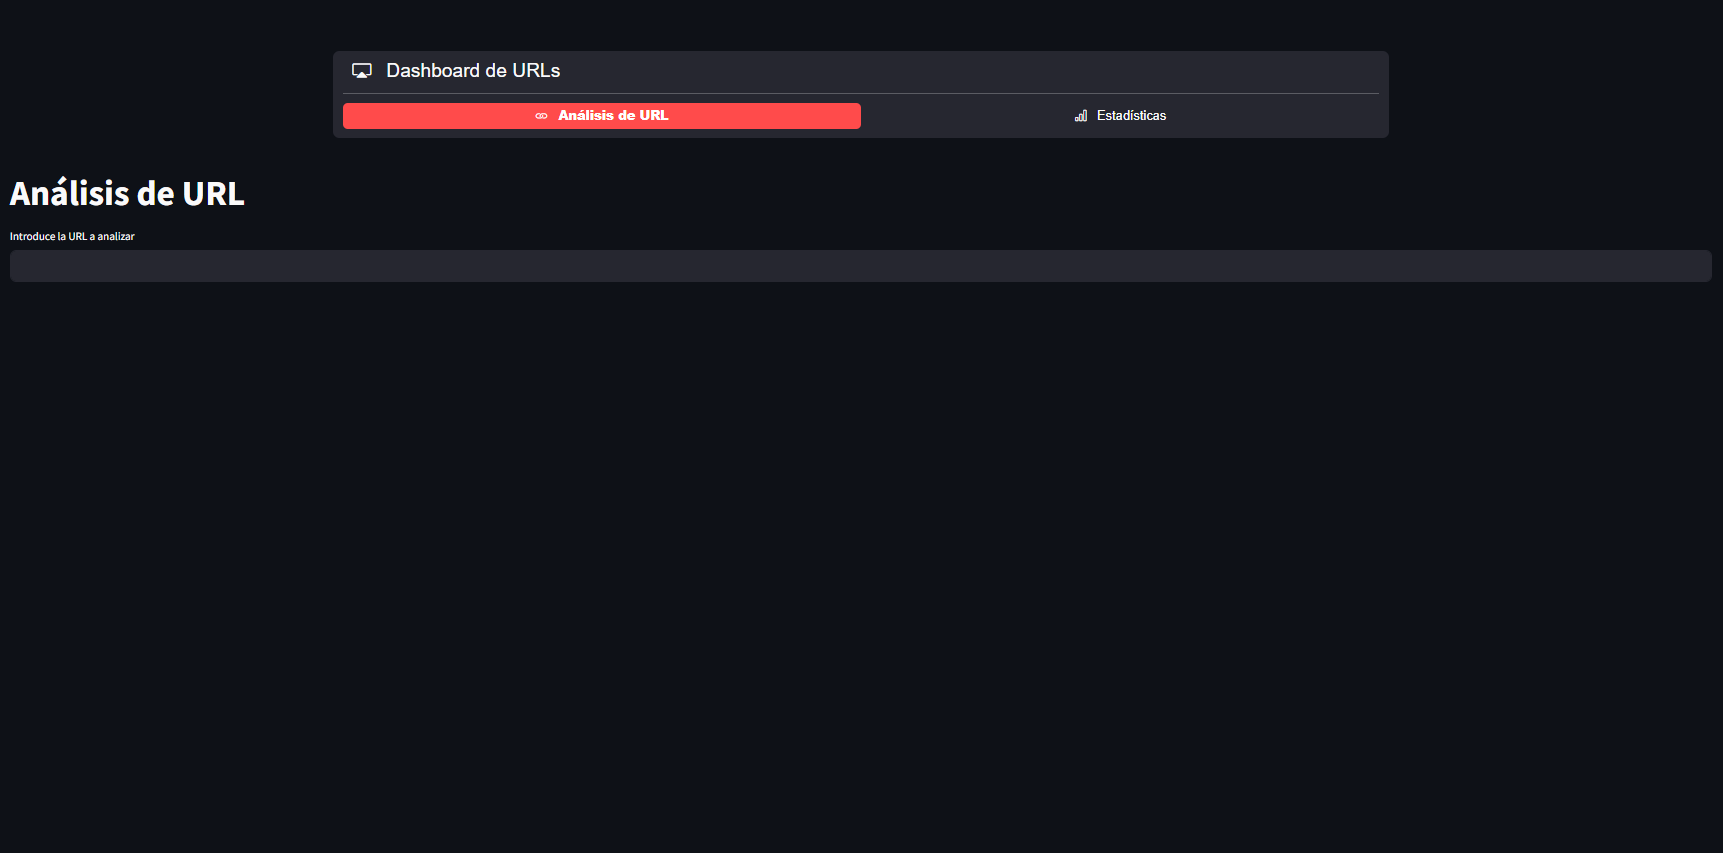
\includegraphics[width=\textwidth]{interfazAnalisis.png}
    \caption{Interfaz de análisis de URL}
\end{figure}

La primera parte del dashboard permite a los usuarios ingresar una URL en un campo de texto. Al presionar el botón de análisis, se extraen diversas características de la URL y se determina su naturaleza maligna o benigna. El informe generado incluye detalles como la longitud de la URL, la cantidad de dígitos y letras, la presencia de subdominios, la entropía del \gls{sld}, y si está registrada o no, entre otros.





\begin{figure}[H]
    \centering
    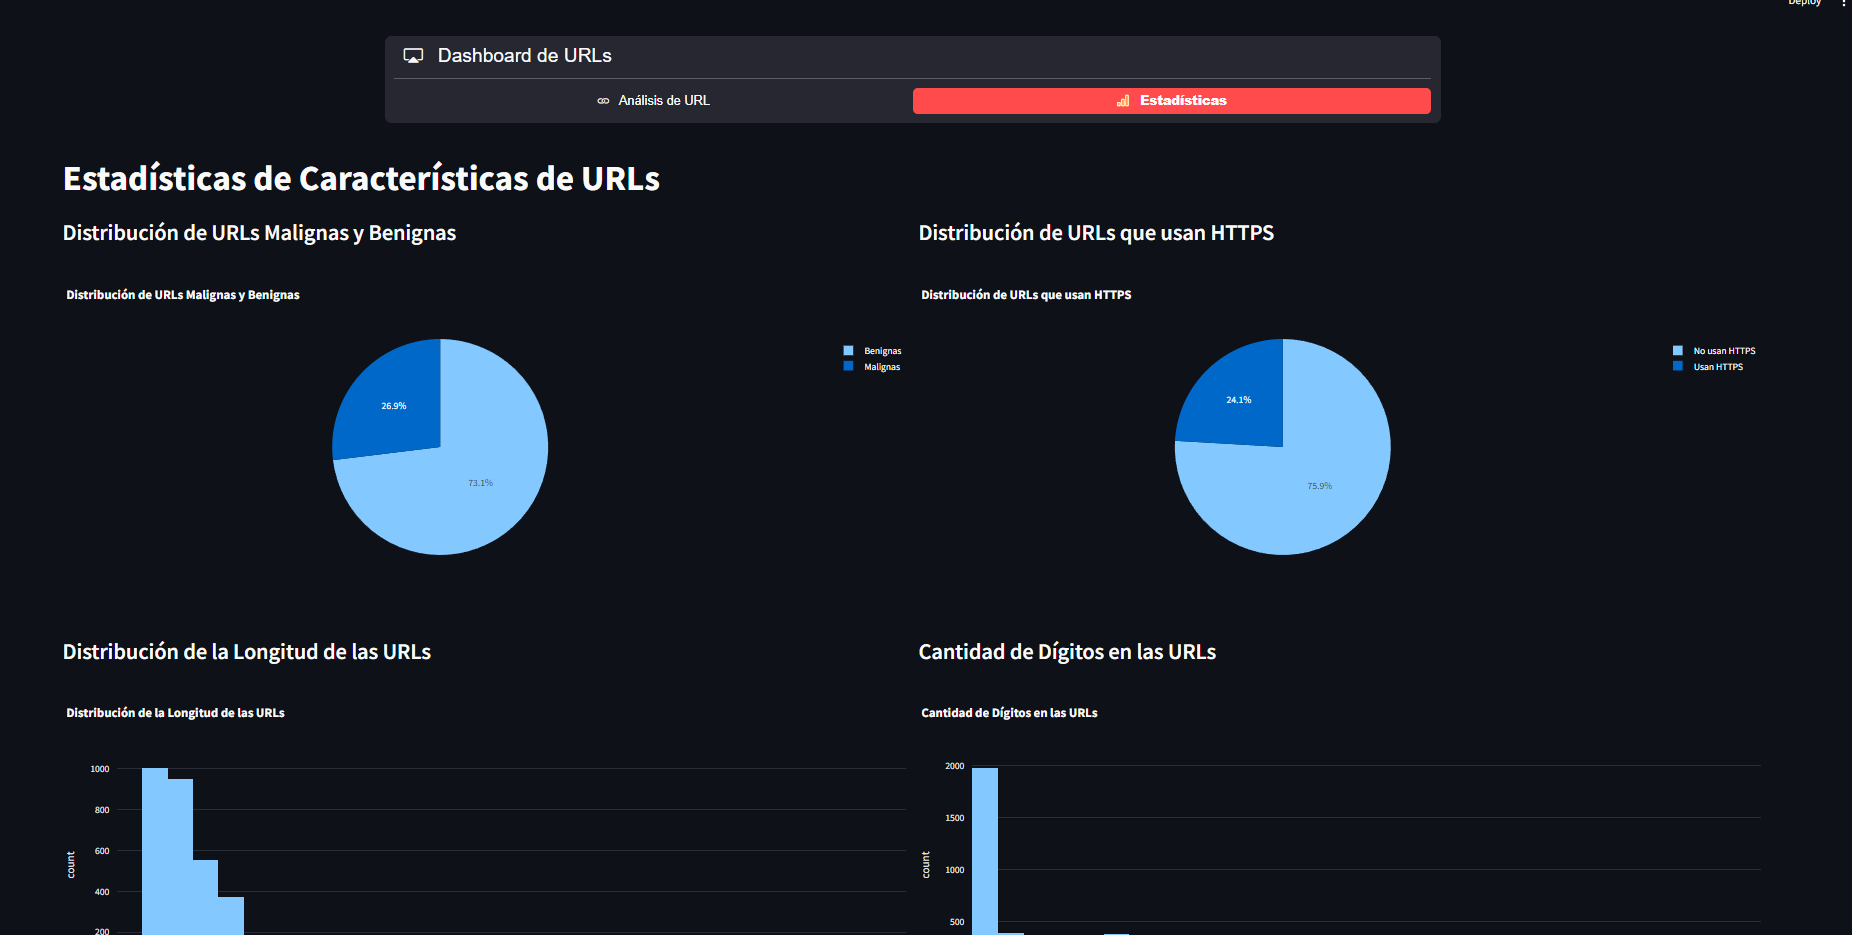
\includegraphics[width=\textwidth]{interfazEstadisticas.png}
    \caption{Vista del dashboard con estadísticas de URLs}
\end{figure}

La segunda parte del dashboard presenta una serie de gráficas que muestran estadísticas derivadas de las características de las URLs almacenadas. Estas gráficas incluyen:

\begin{itemize}
    \item Distribución de URLs Malignas y Benignas.
    \item Distribución de URLs que usan \gls{https}.
    \item Distribución de la Longitud de las URLs.
    \item Cantidad de Dígitos en las URLs.
    \item Cantidad de Letras en las URLs.
    \item Entropía del \gls{sld}.
    \item Distribución de \glspl{tld}.
    \item URLs Registradas y No Registradas.
    \item Edad de los Dominios.
    \item Mapa de Densidad de URLs Benignas y Malignas.
    \item Nube de Palabras de Palabras Sospechosas.
\end{itemize}

\subsection*{Pruebas de Evaluación}

Para evaluar la eficacia y eficiencia del dashboard, se realizaron pruebas en diferentes escenarios. A continuación, se presentan los resultados de estas pruebas:

\subsubsection*{Caso de Prueba 1: Análisis de URL Benigna}


\begin{figure}[H]
    \centering
    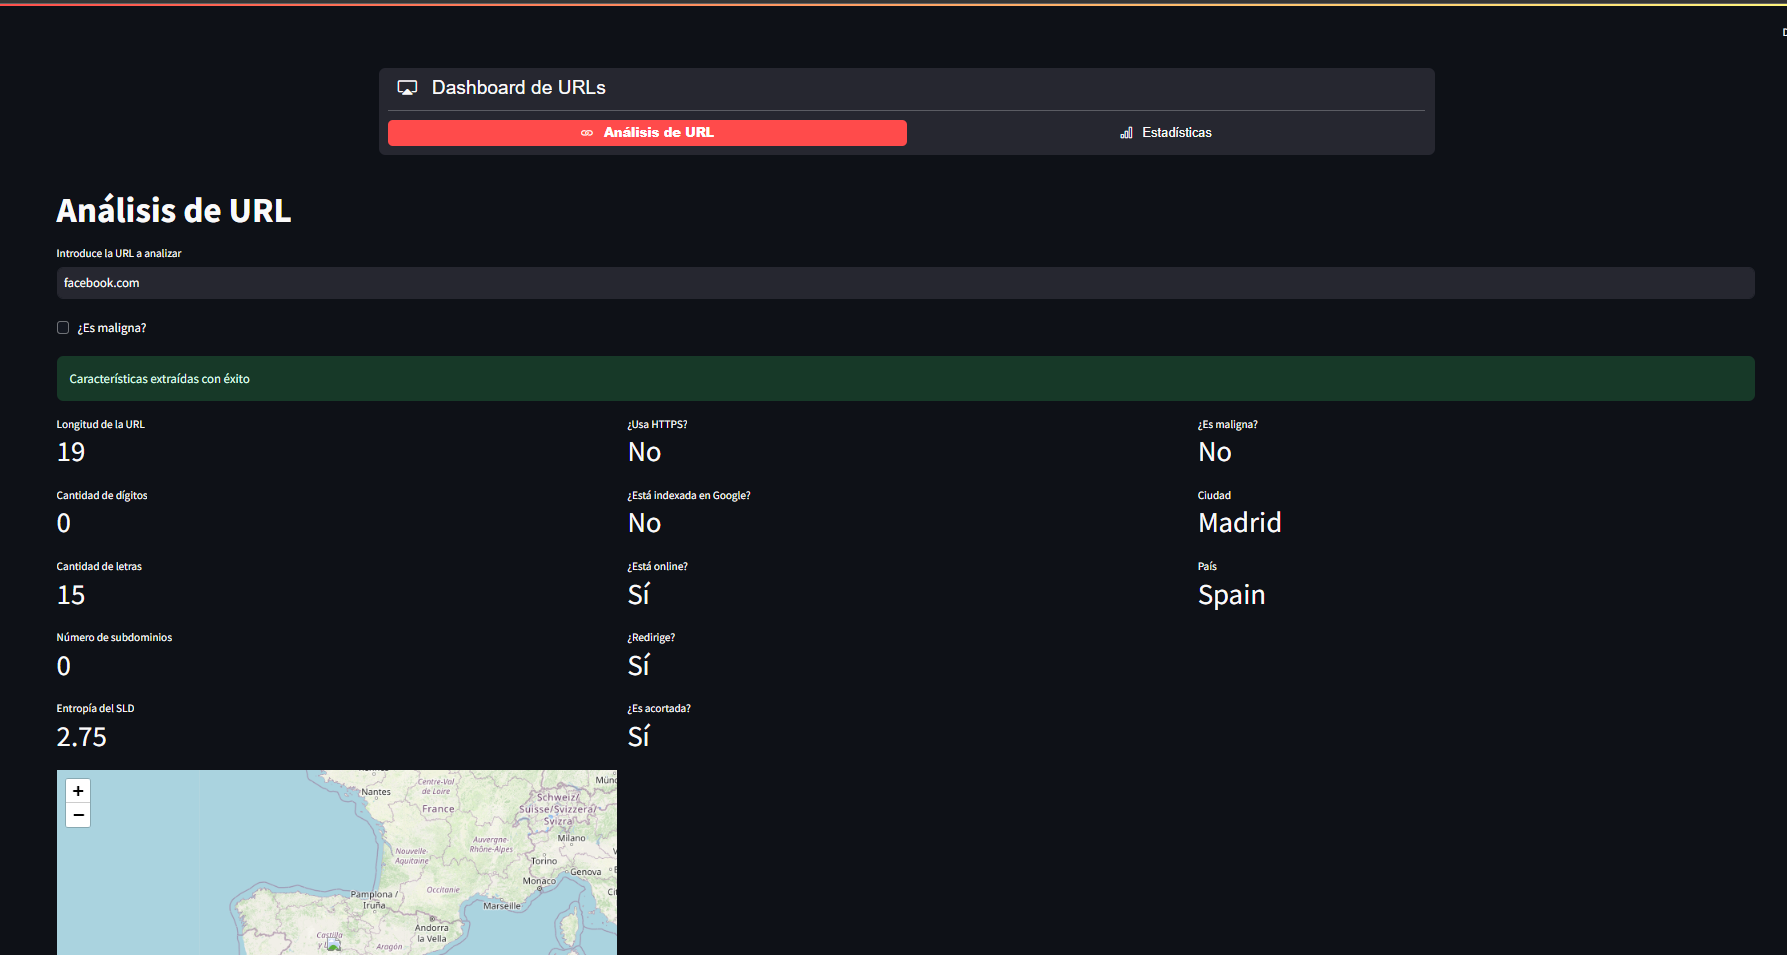
\includegraphics[width=\textwidth]{analisisUrlBenignaDashboard}
    \caption{Análisis de URL Benigna}
\end{figure}

\begin{itemize}
    \item \textbf{Descripción:} Se ingresó la URL de Facebook para el análisis.
    \item \textbf{Resultado:} El dashboard determinó correctamente que la URL es benigna, mostrando las características extraídas.
\end{itemize}



\subsection*{Interactividad y Usabilidad}

El dashboard ofrece una interfaz intuitiva y fácil de usar. Los usuarios pueden obtener información detallada sobre las URLs con solo unos pocos clics. Las gráficas interactivas permiten una exploración profunda de los datos y una mejor comprensión de las características de las URLs almacenadas.


\begin{figure}[H]
    \centering
    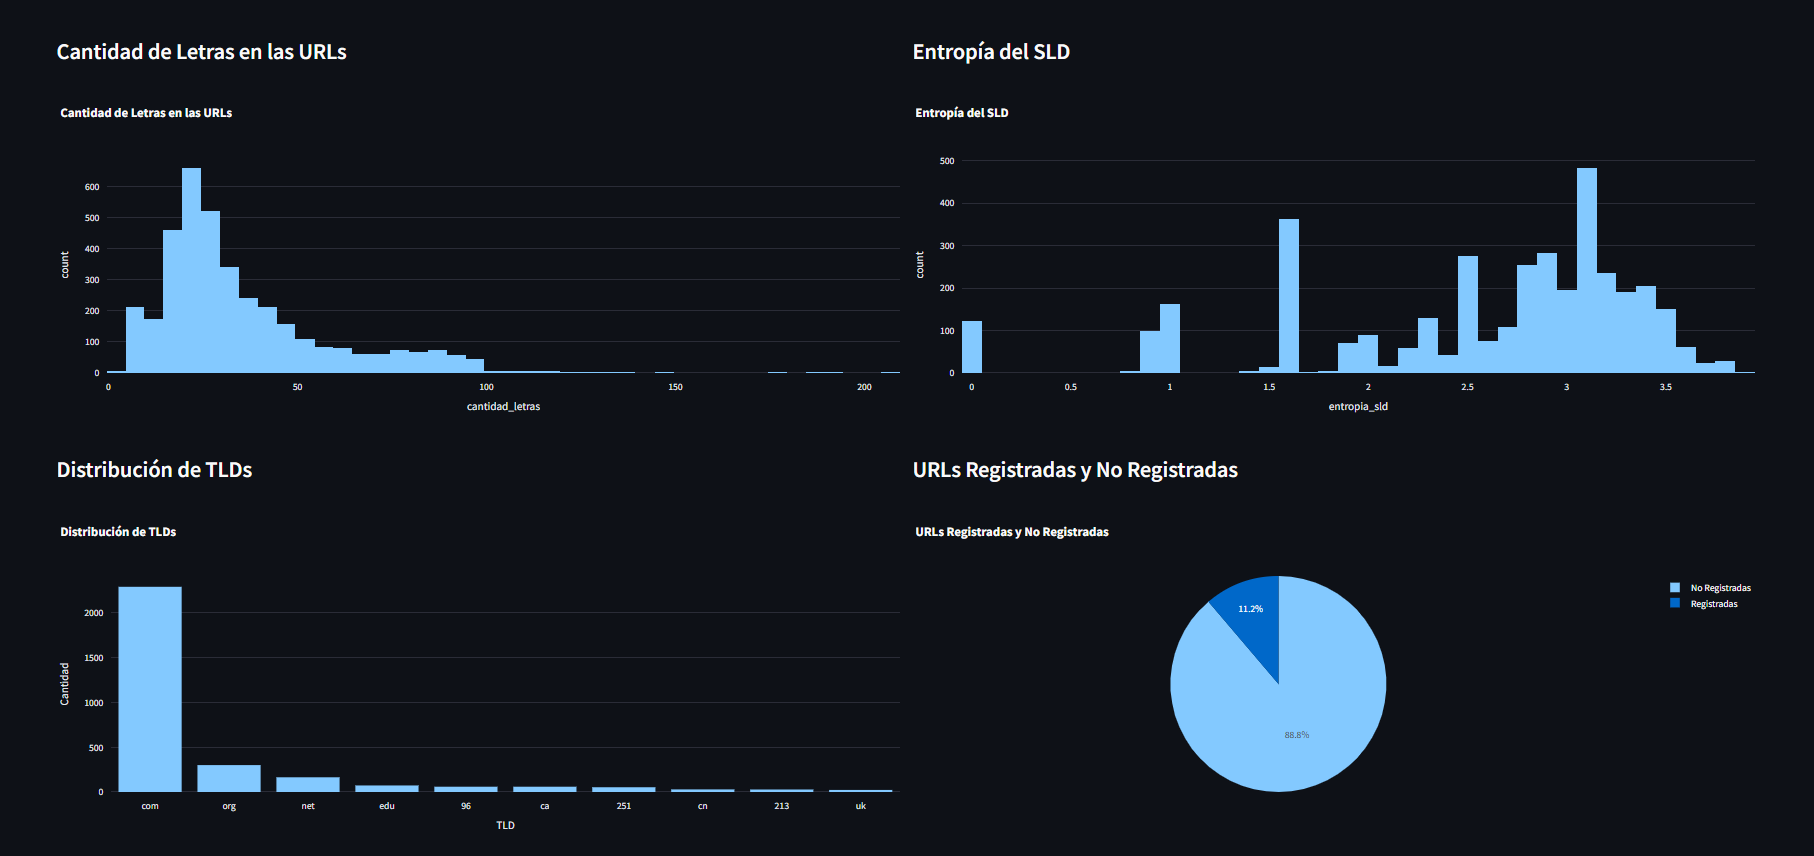
\includegraphics[width=\textwidth]{imageDashboard1.png}
    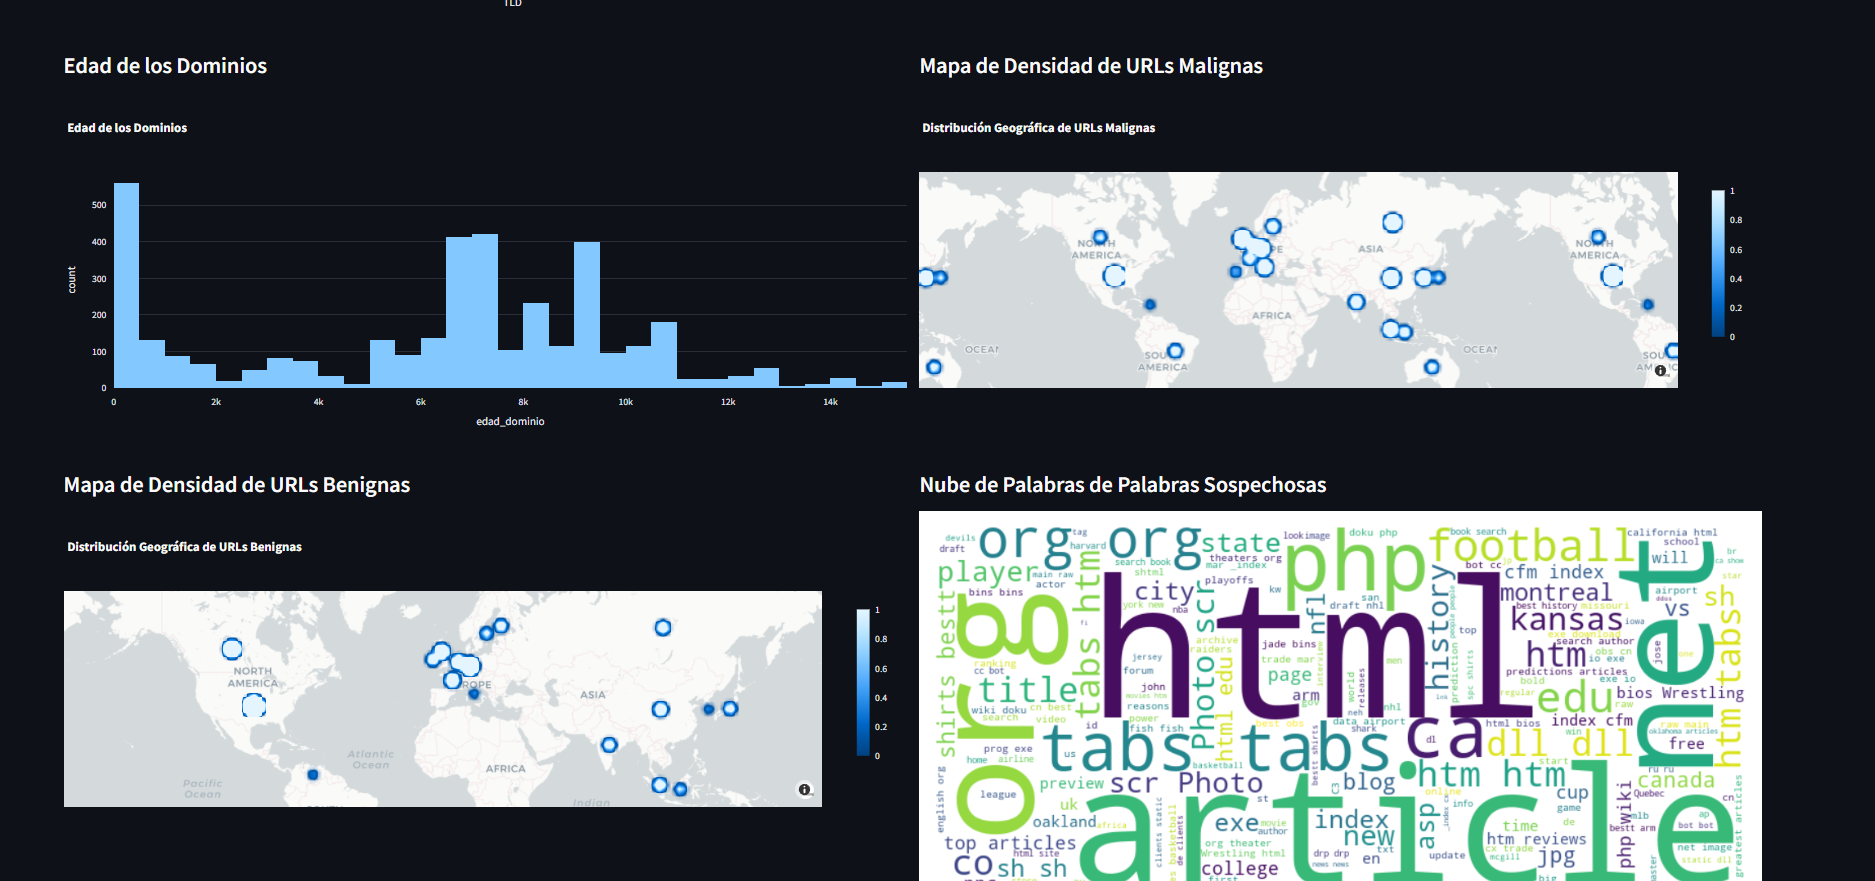
\includegraphics[width=\textwidth]{imageDashboard2.png}
    \caption{Interfaz de análisis de URL interactiva}
\end{figure}

\subsection*{Eficiencia}

El tiempo de respuesta para el análisis de una URL es de aproximadamente 5 segundos, lo cual es razonable dado el nivel de detalle del análisis realizado. Las visualizaciones en el dashboard de estadísticas son rápidas, ya que se basan en datos preextraídos.

\subsection*{Conclusión}

El \textit{Dashboard de URLs} demuestra ser una herramienta efectiva para el análisis y la visualización de características de URLs. Su capacidad para proporcionar informes detallados y visualizaciones interactivas lo convierte en una herramienta valiosa para la evaluación de la seguridad de las URLs.

\subsection*{Consideraciones Adicionales}

\begin{itemize}
    \item \textbf{Interactividad:} Las gráficas interactivas permiten a los usuarios explorar los datos de manera dinámica.
    \item \textbf{Usabilidad:} La interfaz es intuitiva y fácil de navegar.
    \item \textbf{Optimización:} Se pueden considerar mejoras en la velocidad del análisis y la incorporación de funcionalidades adicionales basadas en el feedback de los usuarios.
\end{itemize}

